\documentclass[a4paper,12pt]{article}
\usepackage[spanish]{babel}
\usepackage[T1]{fontenc}
\usepackage[utf8]{inputenc}
\usepackage{url}
\usepackage{graphicx}
\usepackage{listings} %Para poner código fuente
\title{Trabajo final de análisis y diseño de algoritmos I}
\author{Lucas Moauro}
\begin{document}
\maketitle
\newpage
\tableofcontents
\section{Introducción}
% * Motivación para el tp.
% * Resúmen de cambios realizados, aclarar que fue reescrito.
% * Sobre Qt y la SDL(aclarar sobre la complejidad temporal de las estructuras).
% * Resúmen de el contenido de cada sección.
En este informe se presentan las modificaciones al programa Clausula que fueron realizadas como trabajo final
para la cátedra \emph{Análisis y diseño de algoritmos I}.

Clausula \cite{Clausula} es un deductor de lógica de primer orden; a partir de una lista de cláusulas es capaz
de determinar su satisfacibilidad. Además, provee otras funciones útiles para el estudio de lógica como la
unificación de literales y la simplificación de un conjunto de cláusulas utilizando diferentes criterios. Estas funcionalidades
son accesibles a través de una interfaz gráfica intuitiva. Este programa es utilizado por los alumnos de la cátedra \emph{Ciencias de la
computación II} dictada en el segundo año de la carrera.

La motivación del trabajo fue agregar optimizaciones y funcionalidades al programa,
a saber:
\begin{itemize}
\item La refactorización de las clases básicas(Término, Literal, Cláusula, etc). Se agregaron relaciones
de herencia y se cambiaron de lugar métodos.
\item Se cambió la gramática de las clausulas permitiendo identificadores de más de una caracter. Se creó una clase
que provee la adición y eliminación de clausulas y el manejo de errores sintácticos y semánticos.
\item Se creó una clase abstracta que sirve de base para las diferentes estratégias de resolución.
\item Los procedimientos de resolución corren en un hilo de ejecución diferente, lo que permite al usuario detener la resolución sin tener que
salir del programa.
\item Se agregó una regla de inferencia(factorización) que es necesaria para la completitud de los métodos de resolución.
\item Se implementó una simplificación conocida como \emph{simplificación por literales eliminables}.
\item Se implementó una simplificación por subsunción de cláusulas.
\item Se implementó una simplificación de la traza de resolución que elimina las inferencias que no fueron
usadas para derivar la cláusula vacía y se agregó un indexamiento de cláusulas. Esto hace que las pruebas sean
más cortas y legibles.
\item Se integró Clausula con un programa para transformar fórmulas a la forma clausular, lo que permite al usuario
determinar la satisfacibilidad de fórmulas arbitrarias.
\item Se separó completamente la interfaz gráfica de los algoritmos y clases fundamentales, de esta forma
pueden usarse sin mayores dependencias en otros proyectos.
\end{itemize}

\section{Estructuras básicas de lógica de primer orden}
%En esta sección tengo que explicar desde el punto de vista de lógica de primer orden
%a los términos(variables y funciones), literales, y cláusulas. Después hay que describir
%las clases utilizadas para representarlos, sin hacer incapié en como están implementados
%los algoritmos, sólo la interfaz externa. También Sustitución y Argumentos.
En esta sección se describen las estructuras básicas de lógica de primer orden que sirven de base para lós métodos de resolución.
Primero se introducen a partir de su definición en lógica y luego se plantea la correspondencia a los tipos de datos abstractos
y a su implementación a través de las clases de c++ describiendo los métodos más importantes de cada clase. 
Por último, se dan a conocer las estructuras utilizadas para la representación interna de las clases.
\subsection{Términos: Variables y Funciones} %también la clase argumentos
En lógica de primer orden, el conjunto de términos es definido inductivamente \cite{ApuntesLogica}:
\begin{enumerate}
\item Una \emph{variable} es un término.
\item Si $t_1,t_2,...,t_n$ son términos y $f$ es un símbolo de \emph{función}, entonces $f(t_1,t_2,...,t_n)$
  es un término.\footnote{Las constantes son funciones de aridad 0.}
\end{enumerate}
Las variables se caracterizan por tener un identificador y las funciones un identificador y argumentos. La existencia de
dos tipos de términos, sugiere la utilización de un  TDA \emph{Termino} del cual se derivan los TDAs \emph{Variable} y 
\emph{Funcion}.
\begin{center}
\leavevmode
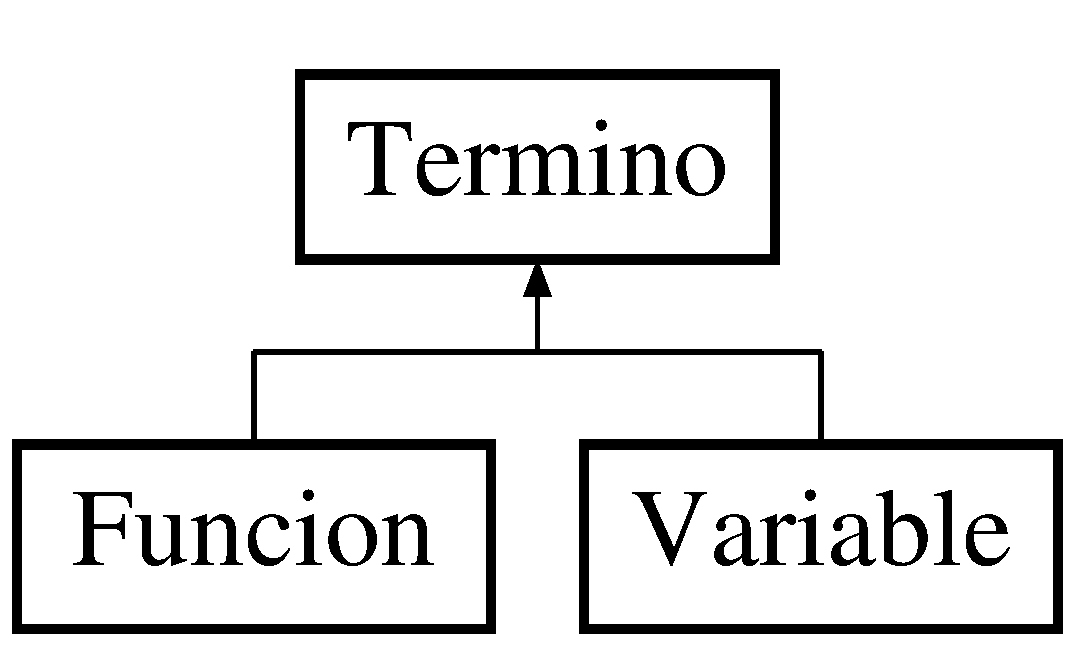
\includegraphics[height=2cm]{imagenes/classTermino}
\end{center}
\subsection{Sustitución}
\subsection{Literal}
\subsection{Cláusula}
\section{Análisis sintáctico de cláusulas} %gramática y parser.
\bibliographystyle{plain}
\bibliography{doc}
\end{document}
